% iris.tex
%
% CS5950 - Machine Learning - Album Covers
%
% This paper covers the results of the our group's experimentation with the
% album covers dataset from the Internet Archive.

\documentclass[11pt,a4paper,titlepage]{article}

\usepackage{geometry}
\geometry{letterpaper}

\usepackage{parskip}
\parindent=0in
\parskip=8pt   % make block paragraphs

\usepackage{hyperref}
\usepackage[utf8]{inputenc}

\usepackage{graphicx}
\usepackage{diagbox}

\usepackage{fancyhdr}
\pagestyle{fancy}

\usepackage{tabularx,ragged2e,booktabs,caption}
\usepackage{amsmath,amsthm,amssymb}
\usepackage{listings}
\usepackage{pdflscape}

\begin{document}

\title{CS5950 - Machine Learning \\
       Identification of Duplicate Album Covers}

\author{Arrendondo, Brandon\\
        Jenkins, James\\
        Jones, Austin\\
        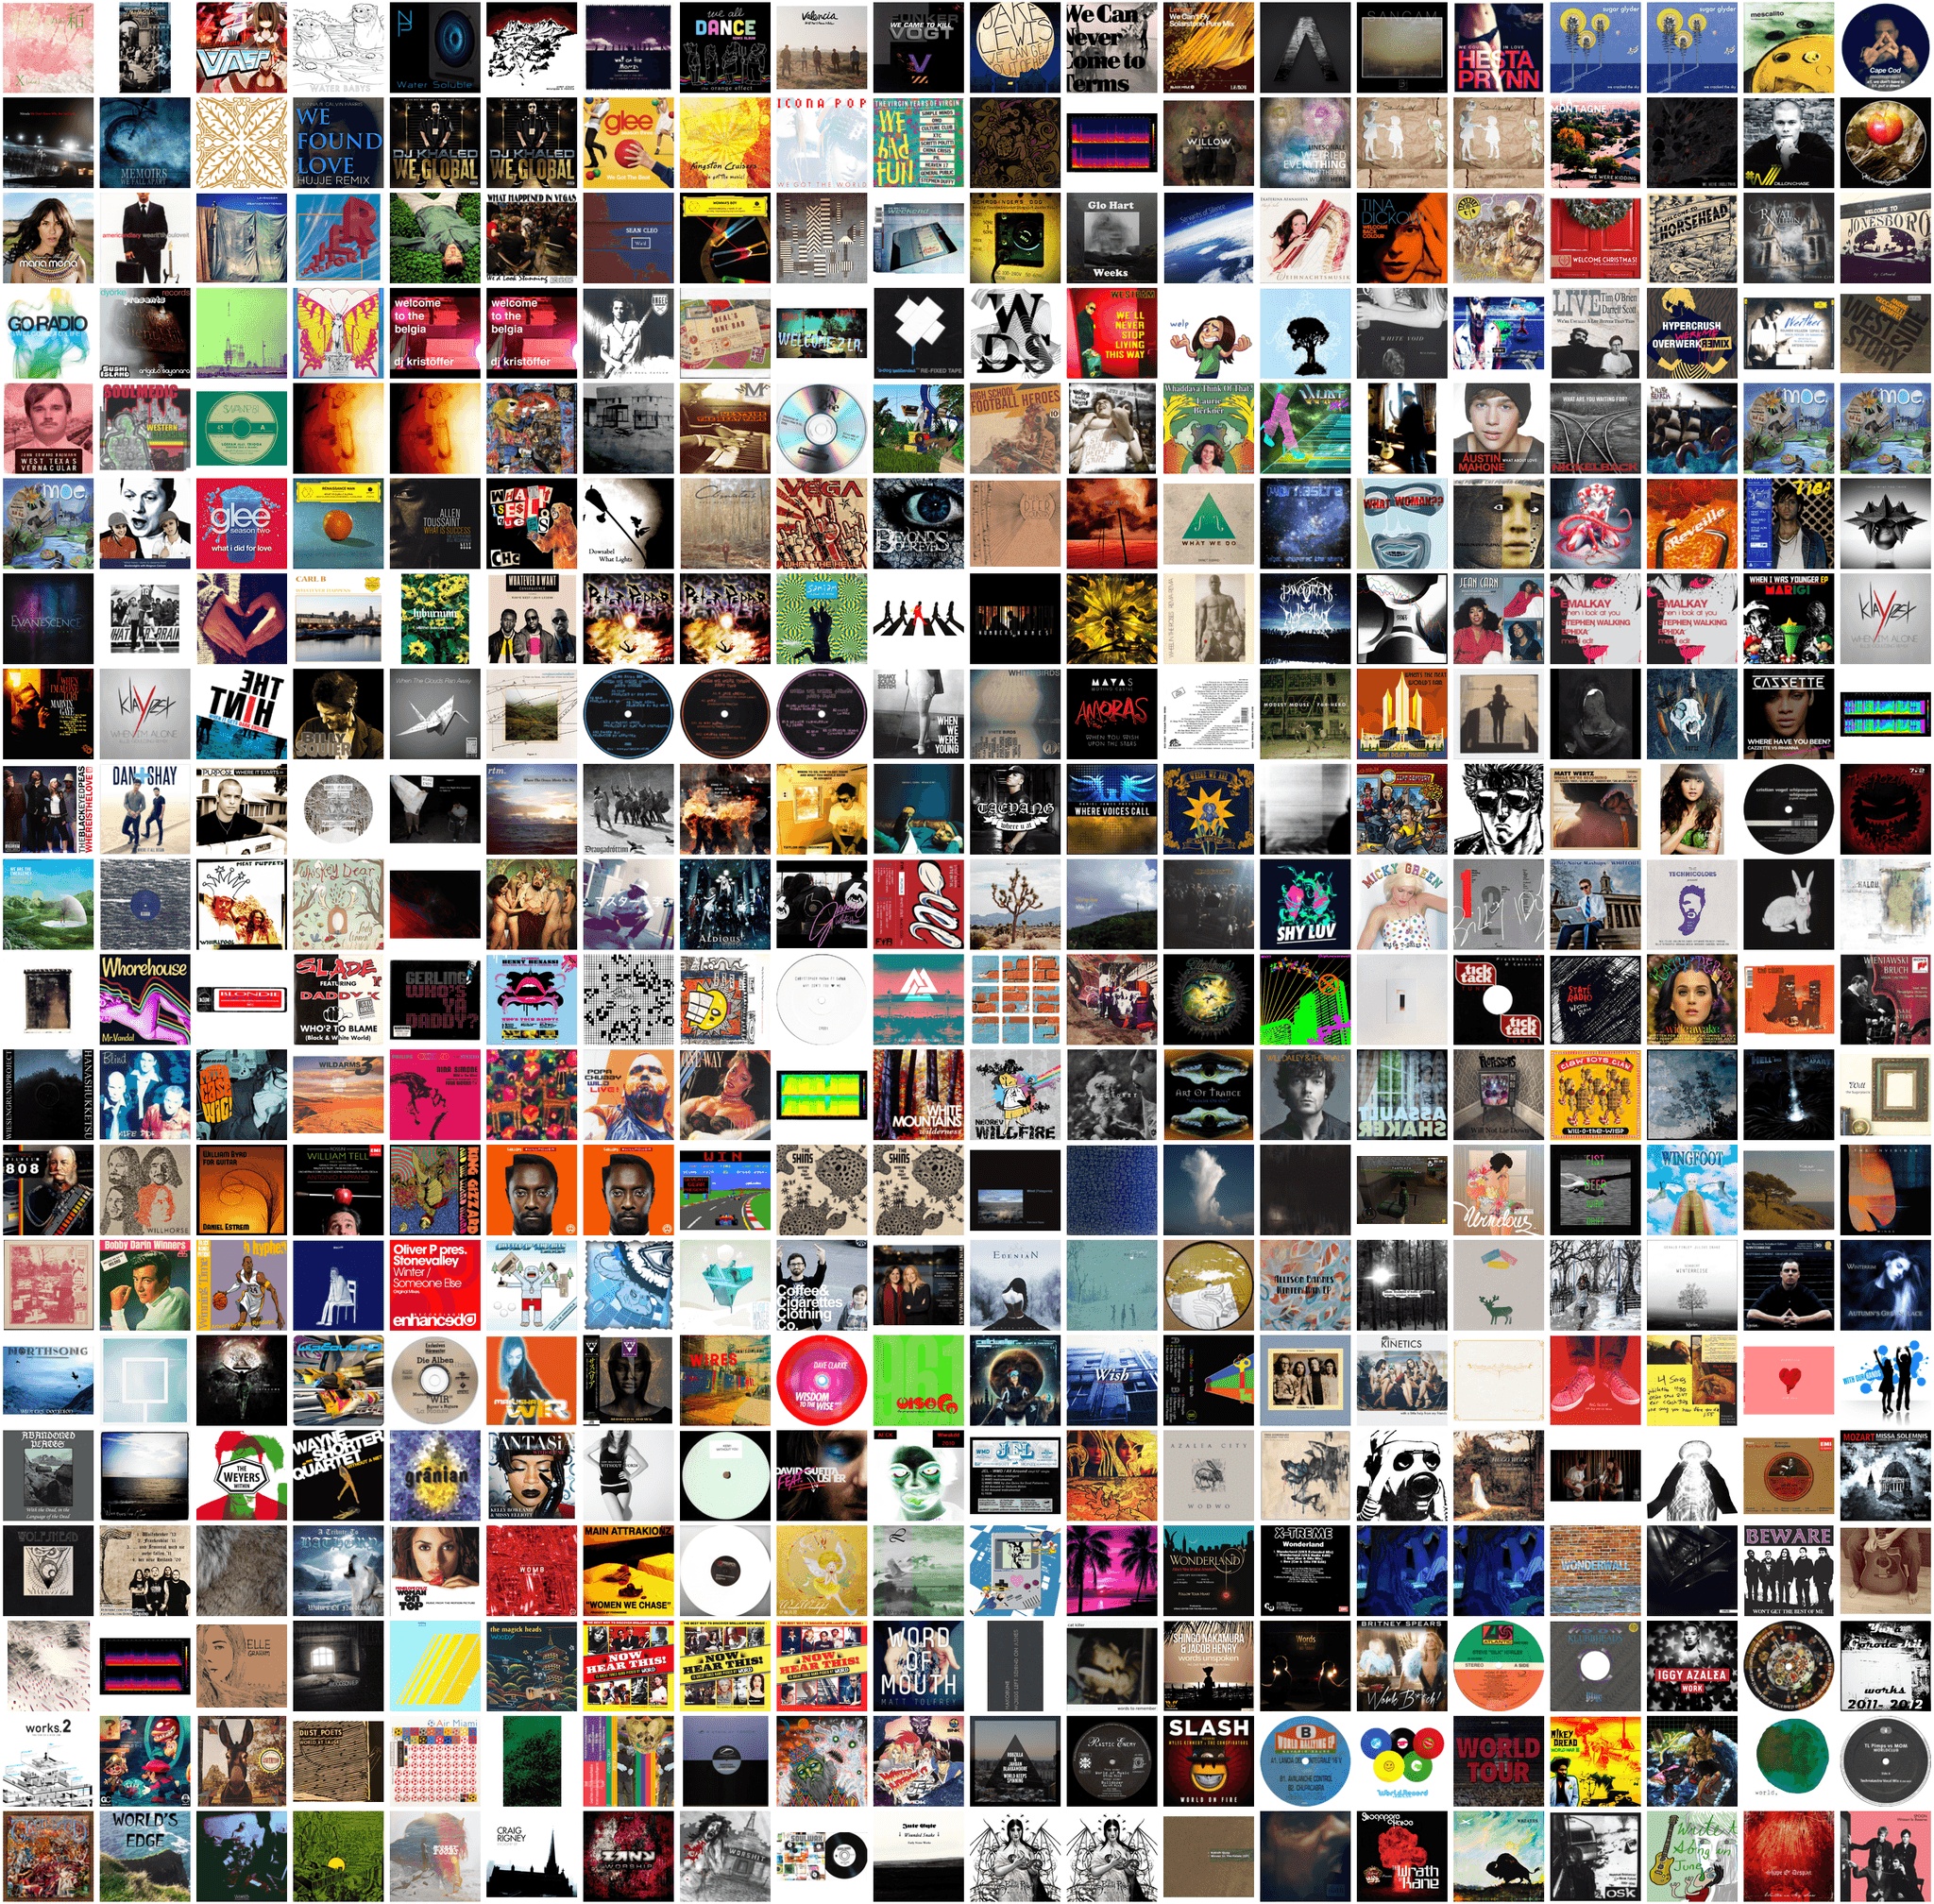
\includegraphics[width=3in]{covers.png}\\[1ex]
    }
\date{\today}

\maketitle

\newpage

\section{Introduction}

This paper covers the results of our groups' initial experimentation with the
album covers dataset from the Internet Archive, located at:

\url{https://blog.archive.org/2015/05/27/experiment-with-one-million-album-covers/}

Every album cover used in this paper is from The Internet Archive and is 
copyright of its respective owners.

The dataset itself contains 997,131 images, which are an assortment of .gif,
.jpg, or .png files.

The goal of our project was to identify images within the dataset that were 
``similar'' to each other, meaning images that were not exactly identical.

\section{First Steps}

Initially, our team searched for existing algorithms that we could implement
that could be used to detect whether two images were similar.  This led us
almost immediately to this site:

\url{http://www.hackerfactor.com/blog/?/archives/432-Looks-Like-It.html}

Most of the ideas in general involved transforming images and converting them
ultimately to a number, which could then be compared, or ``hashing'' the
images.  The two algorithms detailed on the site we refer to as:

\begin{itemize}
    \item
        The Simple Algorithm
    \item
        The DCT (discrete-cosine-transform) Algorithm
\end{itemize}

We will detail these algorithms in the next section.  After having some idea of
algorithms that may work, while implementing the algorithms we also downloaded
the entire dataset onto a computer.

The sizes for each letter directory  are detailed in the table below.  The 
download itself took roughly 1.5 days via the torrent download on the site.

\begin{minipage}{\linewidth}
\centering
\begin{tabular}{|l|l|}
\hline
Directory & Size (GB) \\ \hline
a   & 8.4 \\ \hline
b   & 7.5 \\ \hline
c   & 19 \\ \hline
d   & 7.2 \\ \hline
e   & 4.5 \\ \hline
f   & 5.3 \\ \hline
g   & 4.0 \\ \hline
h   & 5.3 \\ \hline
i   & 5.2 \\ \hline
j   & 1.6 \\ \hline
k   & 2.1 \\ \hline
l   & 7.0 \\ \hline
m   & 7.4 \\ \hline
n   & 4.1 \\ \hline
o   & 3.3 \\ \hline
p   & 5.9 \\ \hline
q   & .380 \\ \hline
r   & 5.0 \\ \hline
s   & 13 \\ \hline
t   & 6.5 \\ \hline
u   & 1.7 \\ \hline
v   & 2.5 \\ \hline
w   & 4.3 \\ \hline
x   & .245 \\ \hline
y   & .769 \\ \hline
the & 9.1 \\ \hline
total & 140  \\ \hline
\end{tabular}
\captionof{table}{Uncompressed Directory Sizes for Album Covers}
\end{minipage}

\section{Initial Complications}

Simply traversing the directory tree was slow and difficult.  A simple command:

\begin{lstlisting}
    ls a/*.png
\end{lstlisting}

Will fail because the size overloads the limit for files returned.  This made a
traditional command fail, like:

\begin{lstlisting}
    md5sum a/*
\end{lstlisting}

We tested several different options, which included:


\begin{itemize}
    \item
        find with exec
    \item
        find with xargs
    \item
        ls -1 with xargs
    \item
        Python script using process pools
\end{itemize}

Using process pools was the fastest method for running our Python-based
implementations of the algorithms.  We used ls with xargs for the md5sums we
ran.

The second major complication was any penalty for bugs.  Because running the hash
across the entire dataset took on the order of half a day, the first few
mistakes took several days to identify and fix.  In hindsight, doing extensive
testing on a smaller dataset is very necessary before running on the entire
dataset.


\section{The Algorithms}

After some initial testing, we were fairly impressed by the algorithms detailed
on:

\url{http://www.hackerfactor.com/blog/?/archives/432-Looks-Like-It.html}

Once again, we refer to them as:

\begin{itemize}
    \item
        The Simple Algorithm
    \item
        The DCT (discrete-cosine-transform) Algorithm
\end{itemize}

We now detail these algorithms in pseudo-code.  Our Python implementation of
these algorithms can be found at:

\url{http://github.com/jpypi/dup-image-search}

\newpage

\subsection{The Simple Algorithm}

\begin{lstlisting}
    simple_hash(image_filepath):

        img = image.load(image_filepath)
        img.resize(8, 8)  # resize the image to 8x8
        img.convert_to_grayscale()
        arithmetic_mean(img.pixels())

        hash = 0  # hash is 64-bit integer
        index = 0
        for each pixel in img.pixels()
            if pixel > mean
                hash.set_bit(index)

            index += 1

\end{lstlisting}

\subsection{The DCT Algorithm}

\begin{lstlisting}
    dct_hash(image_filepath):

        img = image.load(image_filepath)
        img.resize(32, 32)  # resize the image to 32x32
        img.convert_to_grayscale()

        px = img.pixels()

        transformed_matrix = dctII2d(dctII2d(px.transpose()).transpose())
        
        # take the top-left only
        top_left = transformed_matrix.subset(8, 8)

        # leave out [0, 0]
        arithmetic_mean(top_left - top_left[0, 0])

        hash = 0  # hash is 64-bit integer
        index = 0
        for each pixel in img.pixels()
            if pixel > mean
                hash.set_bit(index)

            index += 1

\end{lstlisting}

This algorithm uses the 2D Discrete Cosine Transform, detailed here:

\url{http://en.wikipedia.org/wiki/Discrete_cosine_transform#DCT-II}

Also, per the details found on:

\url{http://www.hackerfactor.com/blog/?/archives/432-Looks-Like-It.html}

The recommendation was to use the top-left only of the transform and to leave
out the [0, 0] term when doing averaging.

\section{Initial Run - Exact Duplicates}

Prior to running our algorithms, first we wanted to reduce the size of the
dataset by removing any corrupt (unloadable) images and any exact duplicates.
For this, we calculated the MD5 hash of each image and used the Python Image
Library (PIL) to verify whether the image was a valid image.

After running this on the dataset (for roughly 10 hours), we were able to
identify matching hashes and calculate that, of the 997,131 images:

\begin{itemize}
    \item
        189,567 images (19\%, 16.65 GB)  were exact duplicates of an image in the remaining set
    \item
        7962 images (about .8\%, 221 MB) images were corrupt
\end{itemize}


\section{Second Run - Simple and DCT Hashes}

After removing the exact duplicates and corrupt images, we then ran each of our
hashes on the full dataset.  After the runs were complete, we compiled the
combined MD5 hash, simple hash, and DCT hash into a SQLite database.  We shared
this database in a Google Drive folder with the team for use in analysis.  We
can make this database publicly available, but it is fairly large (the bzip2
compressed database is 63.2 MB).

\section{Post-run Analysis}

Per the algorithms, any image within hamming distance of five should come close
to matching.  The hamming distance is the number of bit flips two integers are
apart.  To more easily identify all the images within hamming distance of 5 of
any given image, we calculating the hamming weight (the number of ones in the
integer) of each image and stored that in the database as well.

From this, we can say that any image within hamming weight of +/- 5 of the
select image is a candidate for checking the hamming distance.  The problem was
with so many images, checking this takes some time - not a lot - but with about
750,000 images the calculation adds up.

We tried another approach of building up a database slowly and checking with
each insertion if the added image is within 5 of any image already in the
database.  That too, was fairly slow (manageable, but slow).

We decided to refocus, instead, on the determination of what the accuracy for
hamming distance zero was.  It is very easy to calculate the hamming
distance of zero, since we only need to check the database for sets of matching
hashes.

We then built up a list of DCT hashes and simple hashes that, per the
algorithms, should match.  All that was left was to manually verify the
matches.  For this we developed a simple tool that would go through the list
and allow the user to select Yes or No if the images matched.

\begin{minipage}{\linewidth}
    \centering
    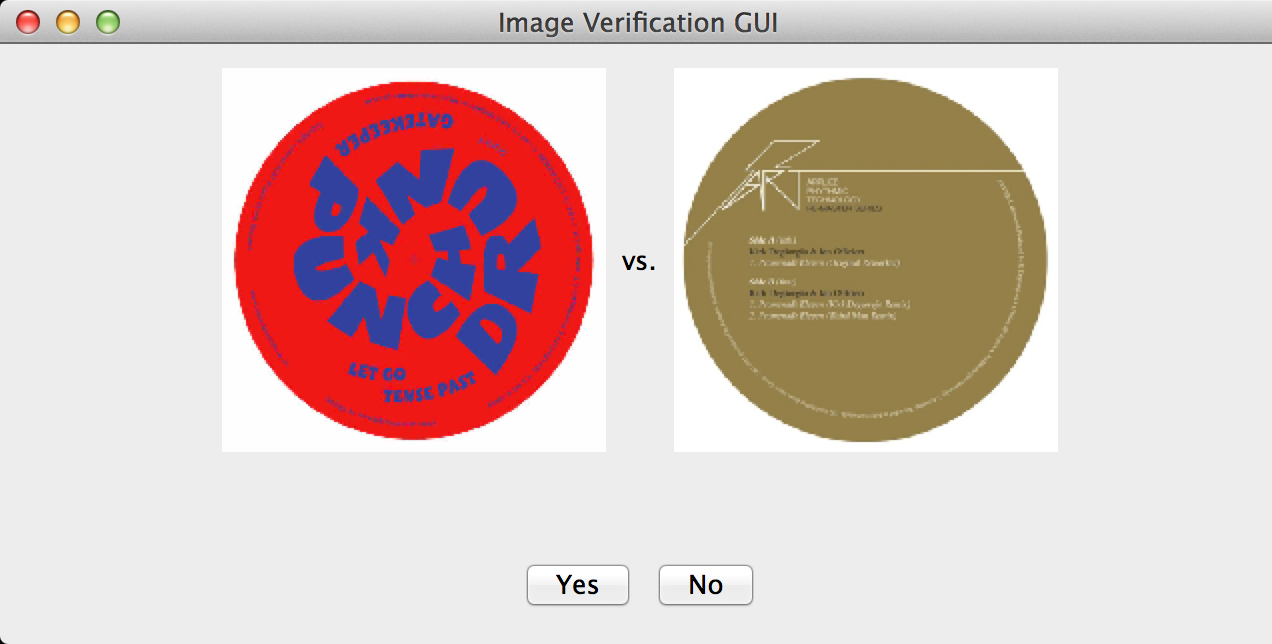
\includegraphics[width=360px]{image_verify.png}
    \captionof{figure}{The Image Verification Tool}
\end{minipage}

The tool writes the results out to a file, which we could then use to determine 
the error rate for false positives.  We also fed this into a database for any
further analysis that would require user input (at least that small subset of
manual user validation would already be done).

We took the matches for simple and matches for DCT and split them into three
for each of us to validate.  We immediately noticed some large sets that were
clearly not matching.  We decided to remove all sets with greater than 4
results as their accuracy was close to 0\%.  We make note of this in the final
numbers.

The final number of sets (between 2 and 5 images each) for the simple algorithm
totalled 9031.  For DCT, the number of sets was 5302.  That was a lot of
pictures to sift through using the tool.  Further tool enhancements would
definitely include:

\begin{itemize}
    \item
        Indication of current progress
    \item
        Keyboard-based entry (in addition to mouse)
    \item
        Ability to go-back and modify a result
\end{itemize}

We all noticed we had a few misclicks here and there, which will contribute to
some error.  Also, each individual had a differing definition of what a
``similar'' album cover would be, which led to some images being accepted by
one person that may not otherwise have been accepted by another.

\section{Results}

\begin{minipage}{\linewidth}
\centering
\begin{tabular}{|l|l|l|l|}
\hline
Images Scanned & Correct & Incorrect & \% Correct \\ \hline
First Set    & 1663    & 2008      & 45.3\% \\ \hline
Second Set   & 1315    & 2546      & 34\% \\ \hline
Third Set    & 1204    & 2378      & 33.6\% \\ \hline
\end{tabular}
\captionof{table}{Results for Simple Algorithm}
\end{minipage}

\begin{minipage}{\linewidth}
\centering
\begin{tabular}{|l|l|l|l|}
\hline
Images Scanned & Correct & Incorrect & \% Correct \\ \hline
First Set       & 1049    & 678      & 60.7\% \\ \hline
Second Set      & 841     & 964      & 46.6\% \\ \hline
Third Set       & 1280    & 420      & 75.3\% \\ \hline
Already Matched & 807     & 49       & 94.2\% \\ \hline
\end{tabular}
\captionof{table}{Results for DCT}
\end{minipage}

The ``Already Matched'' column were images from the database that we had
already manually matched from the Simple algorithm analysis that we did not
have to re-evaluate.  Take note of the fact that we pruned the sets greater 
than 4, which we assume had zero accuracy.

\begin{minipage}{\linewidth}
\centering
\begin{tabular}{|l|l|}
\hline
Algorithm       & Count \\ \hline
Simple          & 14817 \\ \hline
DCT             & 2833  \\ \hline
\end{tabular}
\captionof{table}{Count of Images in Sets Above Length 4}
\end{minipage}

If we were to introduce other algorithms, we should be able to reduce the sets
above 4 to only those that legitimately match.

\begin{minipage}{\linewidth}
\centering
\begin{tabular}{|l|l|}
\hline
Algorithm                           & Percentage Correct \\ \hline
Simple (sets less than 5)                   & 37\%  \\ \hline
DCT (sets less than 5)                      & 81\%  \\ \hline
Simple (assuming sets greater than 4 are 0\%)  & 16\%  \\ \hline
DCT (assuming sets greater than 4 are 0\%)     & 45\%  \\ \hline
\end{tabular}
\captionof{table}{Combined Results for Each Algorithm}
\end{minipage}

Finally, we ran the results for first taking the simple hash and then only
predicting the files were similar if the DCT hashes also matched.

\begin{minipage}{\linewidth}
\centering
\begin{tabular}{|l|l|l|}
\hline
Correct & Incorrect & \% Correct \\ \hline
1817    & 100      & 94.7\% \\ \hline
\end{tabular}
\captionof{table}{Results for Simple Then DCT}
\end{minipage}

It is worth noting that the accuracy was higher than either algorithm alone,
however the number of duplicates found overall was smaller, which would lead to
more false-negatives (which we did not measure).

\section{Analysis of Results}

We gained great insight into what the algorithms did and did not see once
seeing the images that had matching hashes.

The failing points we saw in the algorithms were:

\begin{itemize}
    \item
        The algorithms are color-insensitive.  As a result, covers that differ
        only by color were identified (incorrectly) as matches.

    \item
        Small details are not picked up in the algorithm.  This includes, for
        the most part, any text.  This had three weak points:

        Many album covers were not covers but rather images of the
        CD/record.  As a result, the round circular image dominated the
        algorithm and the text to distinguish album covers was the only
        thing that could differentiate them.  A large number of false
        positives were due to this.

        There were many ``compilation'' albums, in particular Glee
        albums and ``The Voice'' albums, whose only differentiating
        feature was the song name on the album cover.  Those were
        always matching, which led to a large number of false
        positives.

        Some albums by the same producer had matching artwork but
        different artists/songs.  The text was, again, a differentiator
        here and did not get picked up by either algorithm.
\end{itemize}

Despite the failings, the algorithms were good (at hamming distance zero) of
detecting a number of duplicates.

\section{Recommendations}

Based on what we saw, we would recommend using the DCT algorithm as a first
pass (after exact duplicates were removed with MD5), then another algorithm be
applied to determine:

\begin{itemize}
    \item
        Shape - if it is a circular picture it is likely an image of the album
        itself (and not a cover).  If character recognition is expensive, apply
        it to these hits first.
    \item
        Color - Again, if the DCT algorithm indicates the images are close,
        then some color-matching algorithm would help to weed out
        false-positives.
\end{itemize}

\section{Next Steps}

If we were to continue working on this, we would recommend first the use of a
character-recognition algorithm to help sort out false-positives.

We would also tune the image verification program, likely refactoring it as a
web page for detecting if the images are equal, to distribute the workload
better.  We would feed the results directly into a database.

This is also a project which lends itself readily to some massive
parallelization step - divide and conquer works well on this as many of the
steps are independent (like the individual image hashing).  Per some of our
discussions, offloading much of the image processing work to a graphics
processor would likely significantly speed up the algorithms, as they are
tailored to doing these kinds of transformations.

We would also map out the accuracy for hamming weights 1, 2, 3, and 4, to see
how rapid the decline in accuracy is.  Honestly, this is what we ran out of time
to do - in hindsight we would have worked with much smaller datasets first as a
training step before moving to the full dataset for testing.

\end{document}
